\documentclass[11pt]{article}
\usepackage[margin=1in]{geometry}
\usepackage{booktabs}
\usepackage{float}
\usepackage{graphicx}
\usepackage{hyperref}
\usepackage{setspace}

\hypersetup{hidelinks}
\setstretch{1.1}

\title{Econ 5253 Problem Set 6}
\author{Last Name: Cheng}
\date{March 24, 2026}

\begin{document}
\maketitle

\section*{Data Choice}
For this problem set, I used the
\href{https://raw.githubusercontent.com/owid/co2-data/master/owid-co2-data.csv}{Our World in Data CO2 dataset}.
I chose this dataset because I am interested in the relationship between economic development, energy use, and carbon emissions.
The file contains country-year observations for emissions, energy, population, and GDP, which makes it well suited for both data cleaning and visualization.

\section*{Cleaning and Transformation}
I downloaded the raw CSV directly in Python and cleaned it with \texttt{pandas}.
The main cleaning steps were:
\begin{enumerate}
\item I kept only rows with a three-letter ISO country code, which removes aggregate regions and other non-country entities.
\item I restricted the sample to 1990 and later so that the visualizations focus on the modern period.
\item I identified 2022 as the latest year with broad coverage for all variables needed in the cross-sectional plots. The raw dataset extends to 2024, but GDP values needed for the income-emissions comparison are missing for 2023 and 2024.
\item I created GDP per capita by dividing GDP by population.
\item I constructed source shares for national CO2 emissions from coal, oil, gas, cement, flaring, and other industry.
\item For the bubble chart, I kept only countries with population of at least 10 million and non-missing values for GDP per capita, CO2 per capita, and coal share.
\end{enumerate}

After cleaning, the working dataset contains 7,194 observations across 218 countries for the years 1990--2022.
All of these steps are fully reproducible in \texttt{PS6\_Cheng.py}.

\section*{Visualizations}

\begin{figure}[H]
\centering
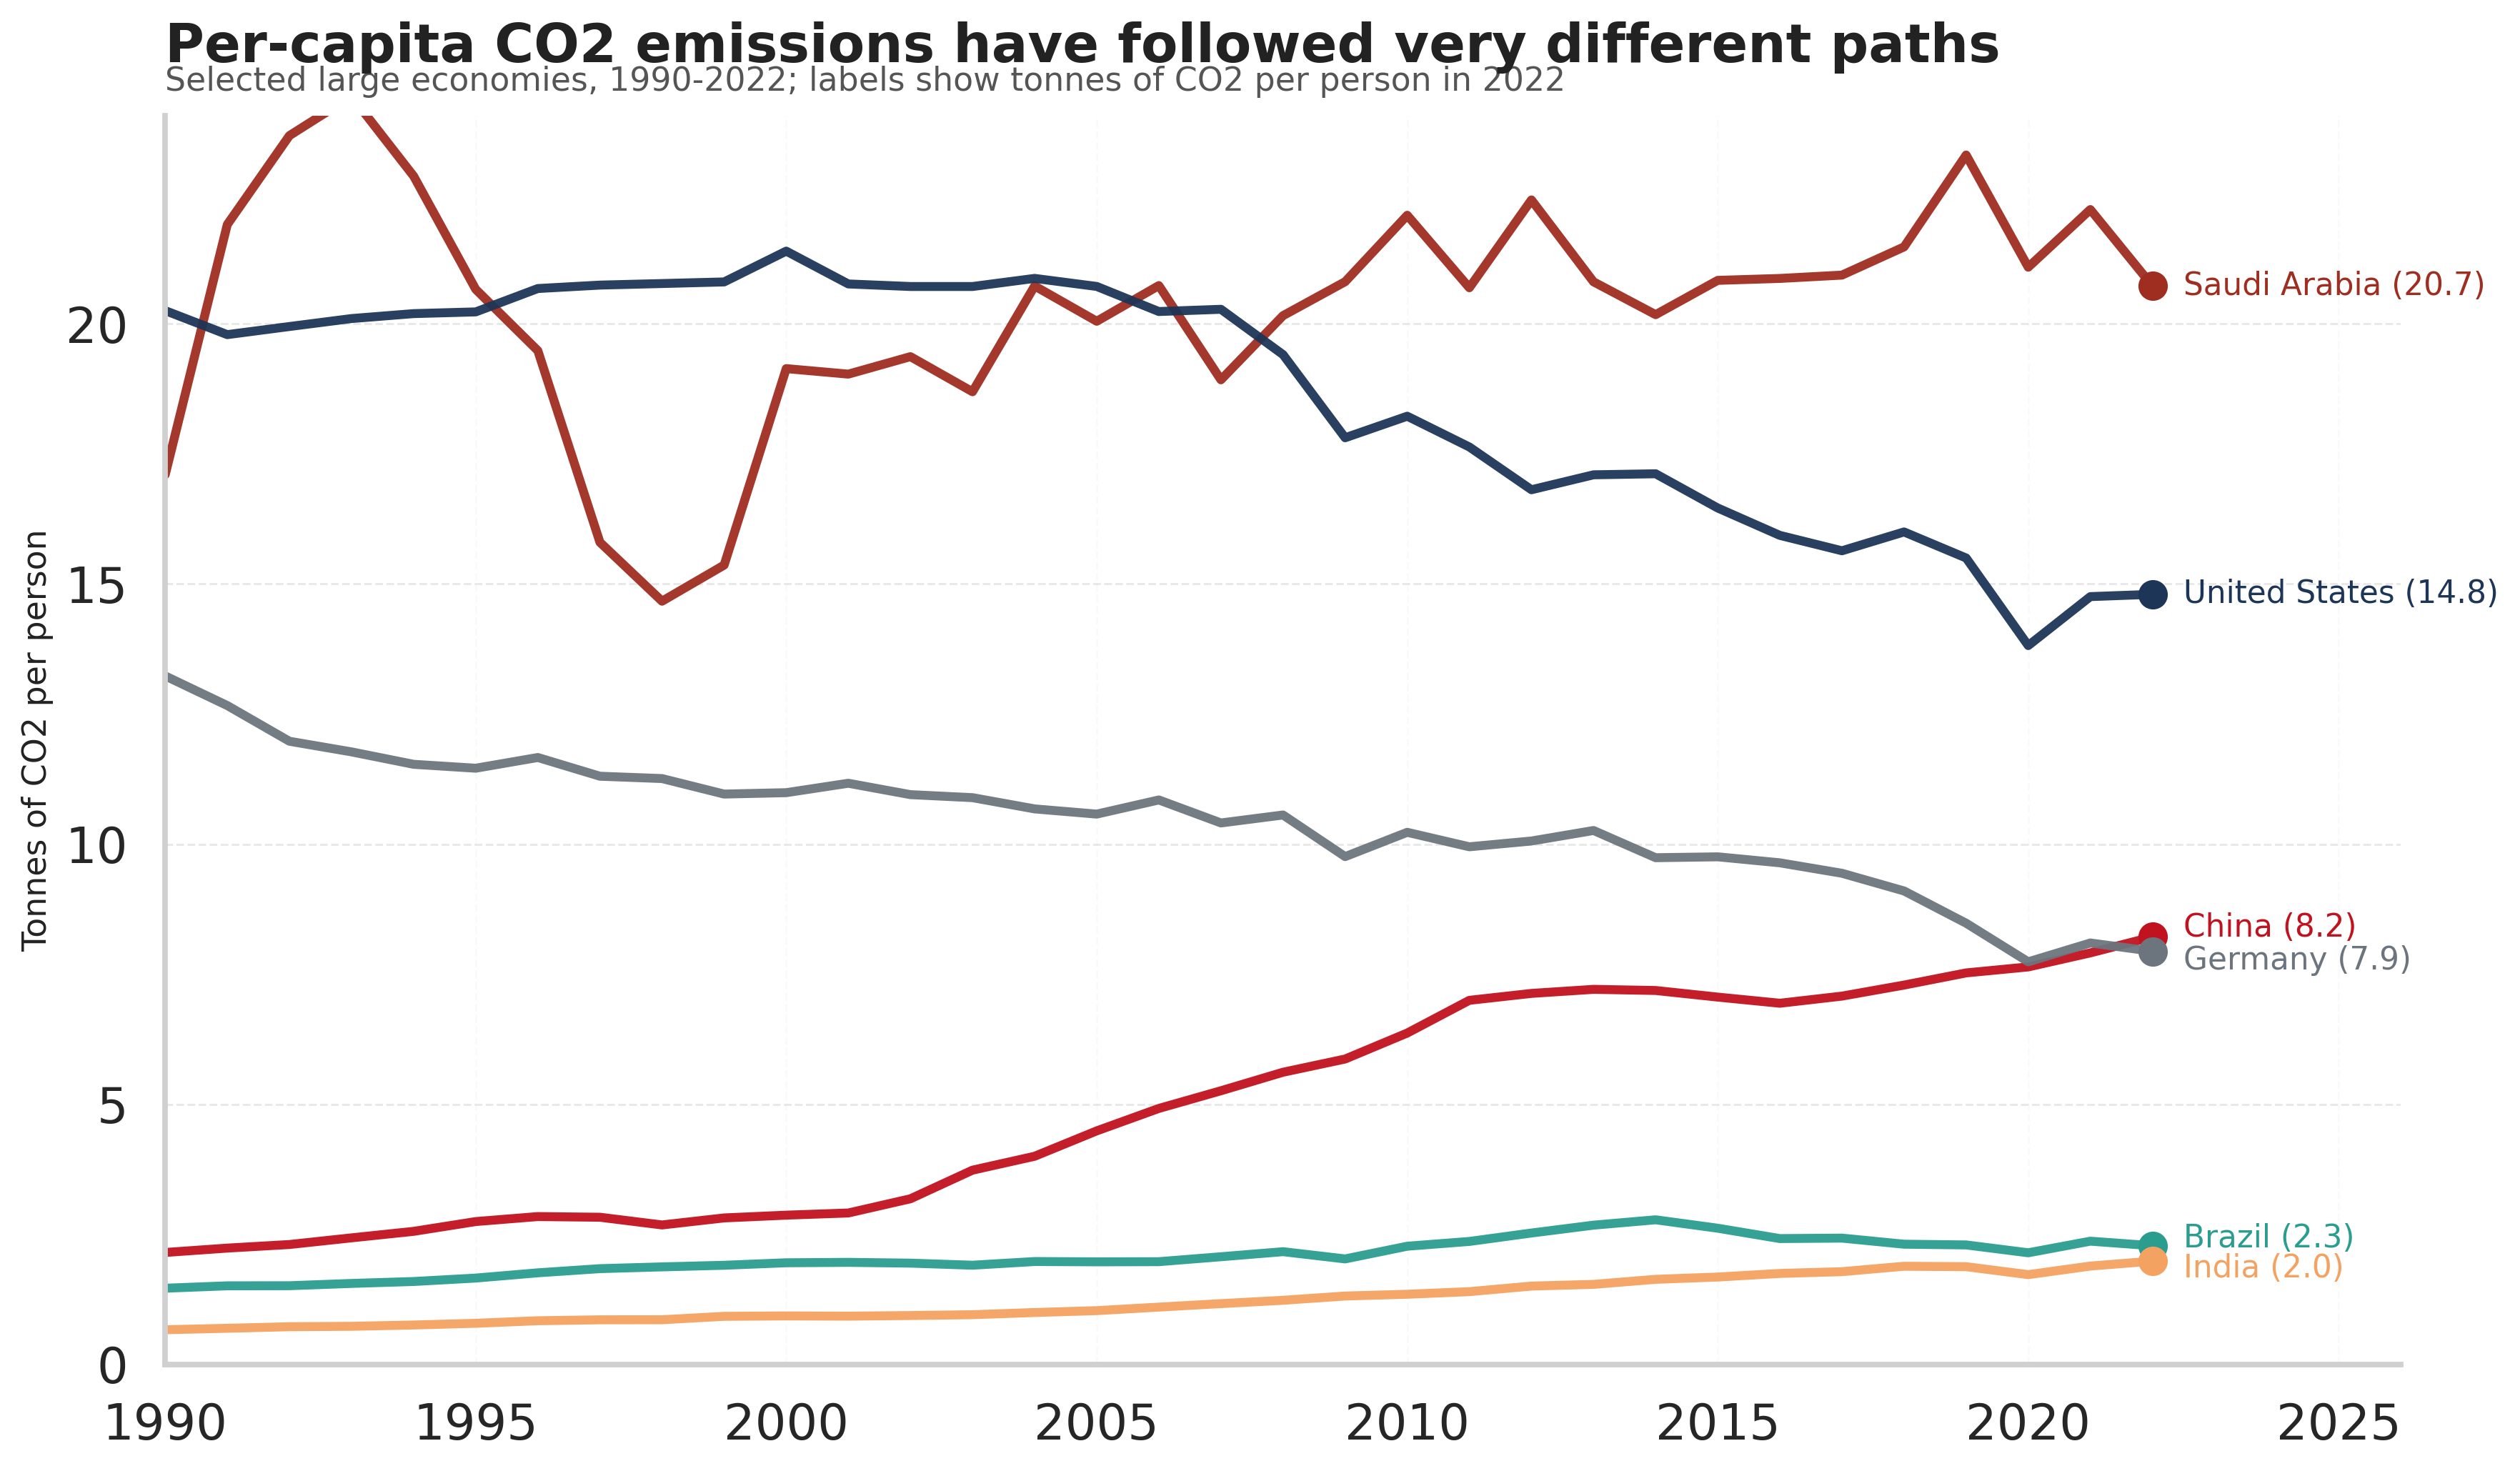
\includegraphics[width=\textwidth]{PS6a_Cheng.png}
\caption{Per-capita CO2 emissions for selected large economies, 1990--2022.}
\end{figure}

Figure 1 shows that countries with large economies do not follow a common emissions path.
The United States and Germany both reduced emissions per person over time, while China and India increased as industrialization and energy demand expanded.
Saudi Arabia remains at a very high emissions level throughout the sample, and Brazil stays comparatively low.
This figure is helpful because it makes the time dimension clear: total emissions alone would hide the fact that the trajectories differ dramatically once population is taken into account.

\begin{figure}[H]
\centering
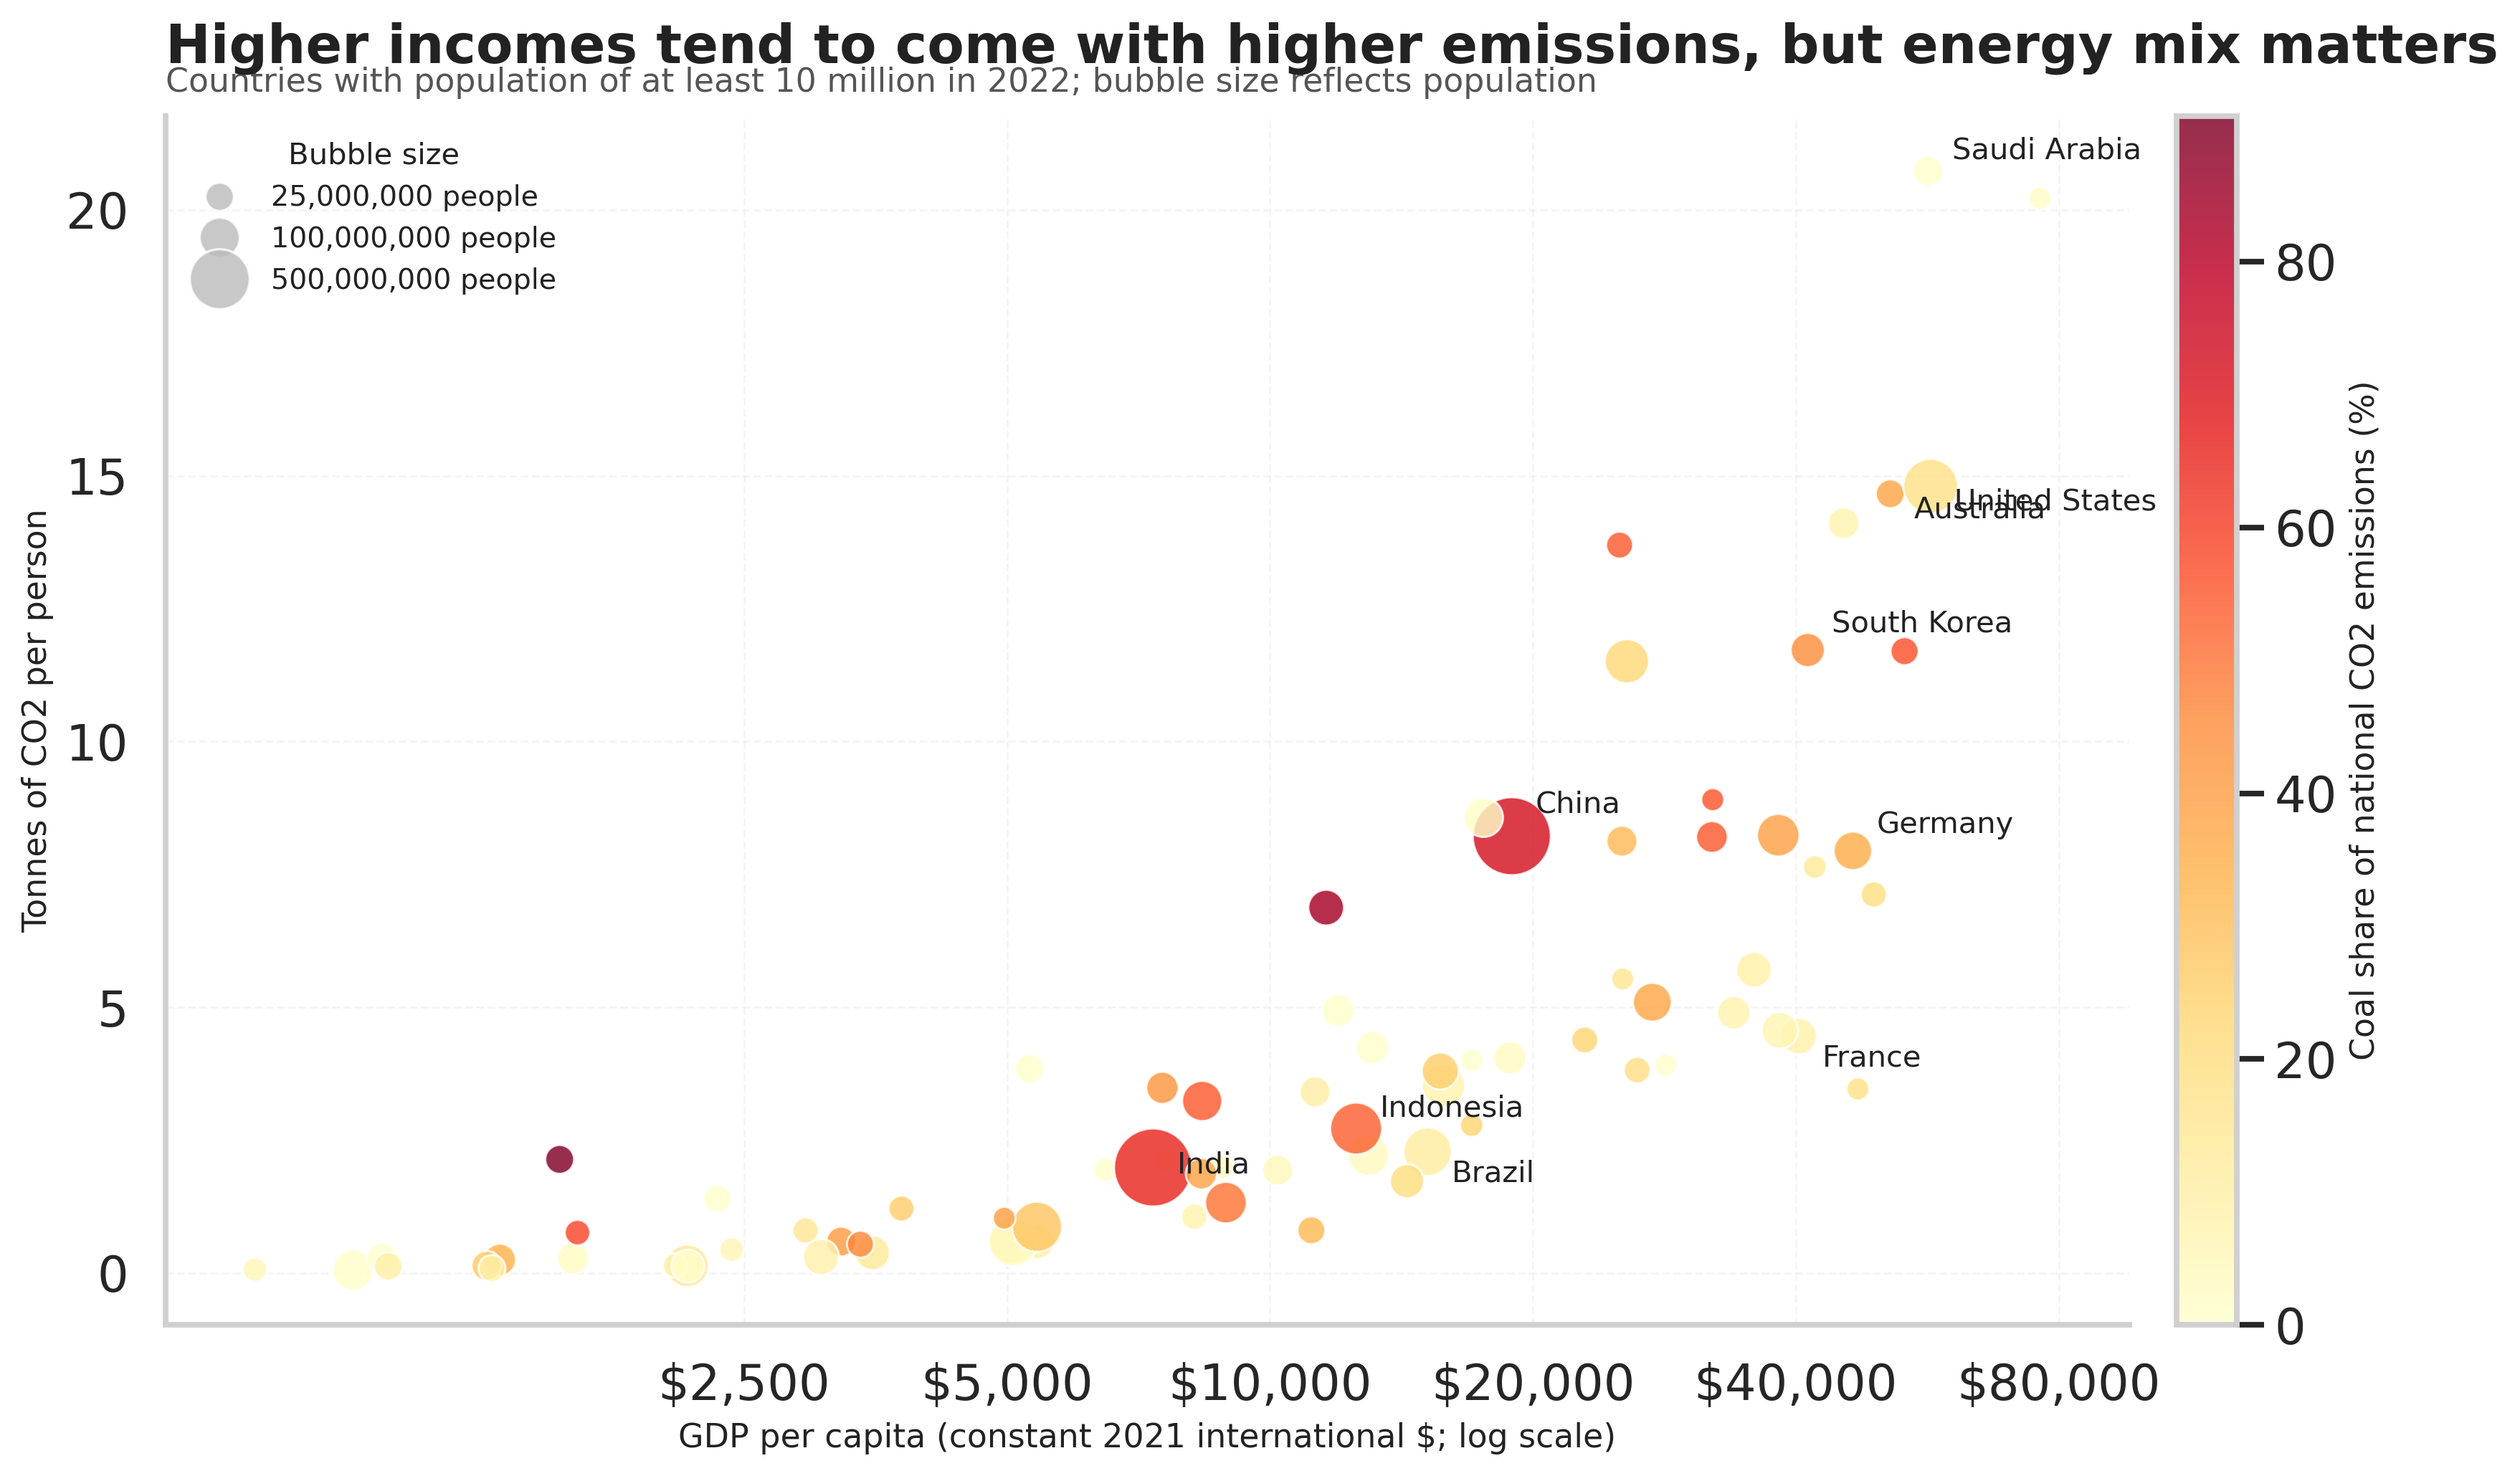
\includegraphics[width=\textwidth]{PS6b_Cheng.png}
\caption{GDP per capita and CO2 per capita in the latest complete year, with bubble size proportional to population and color showing coal dependence.}
\end{figure}

Figure 2 compares income and emissions across countries in 2022.
There is a visible positive relationship between GDP per capita and CO2 per capita, but the scatter also shows that countries with similar income levels can have very different emissions outcomes.
For example, France emits much less per person than the United States even though both are high-income economies, while Saudi Arabia combines high income with extremely high emissions.
The color scale adds another layer of information by showing that coal-heavy energy systems are often associated with higher emissions.
This figure is useful because it shows both the broad development-emissions relationship and the importance of energy mix.

\begin{figure}[H]
\centering
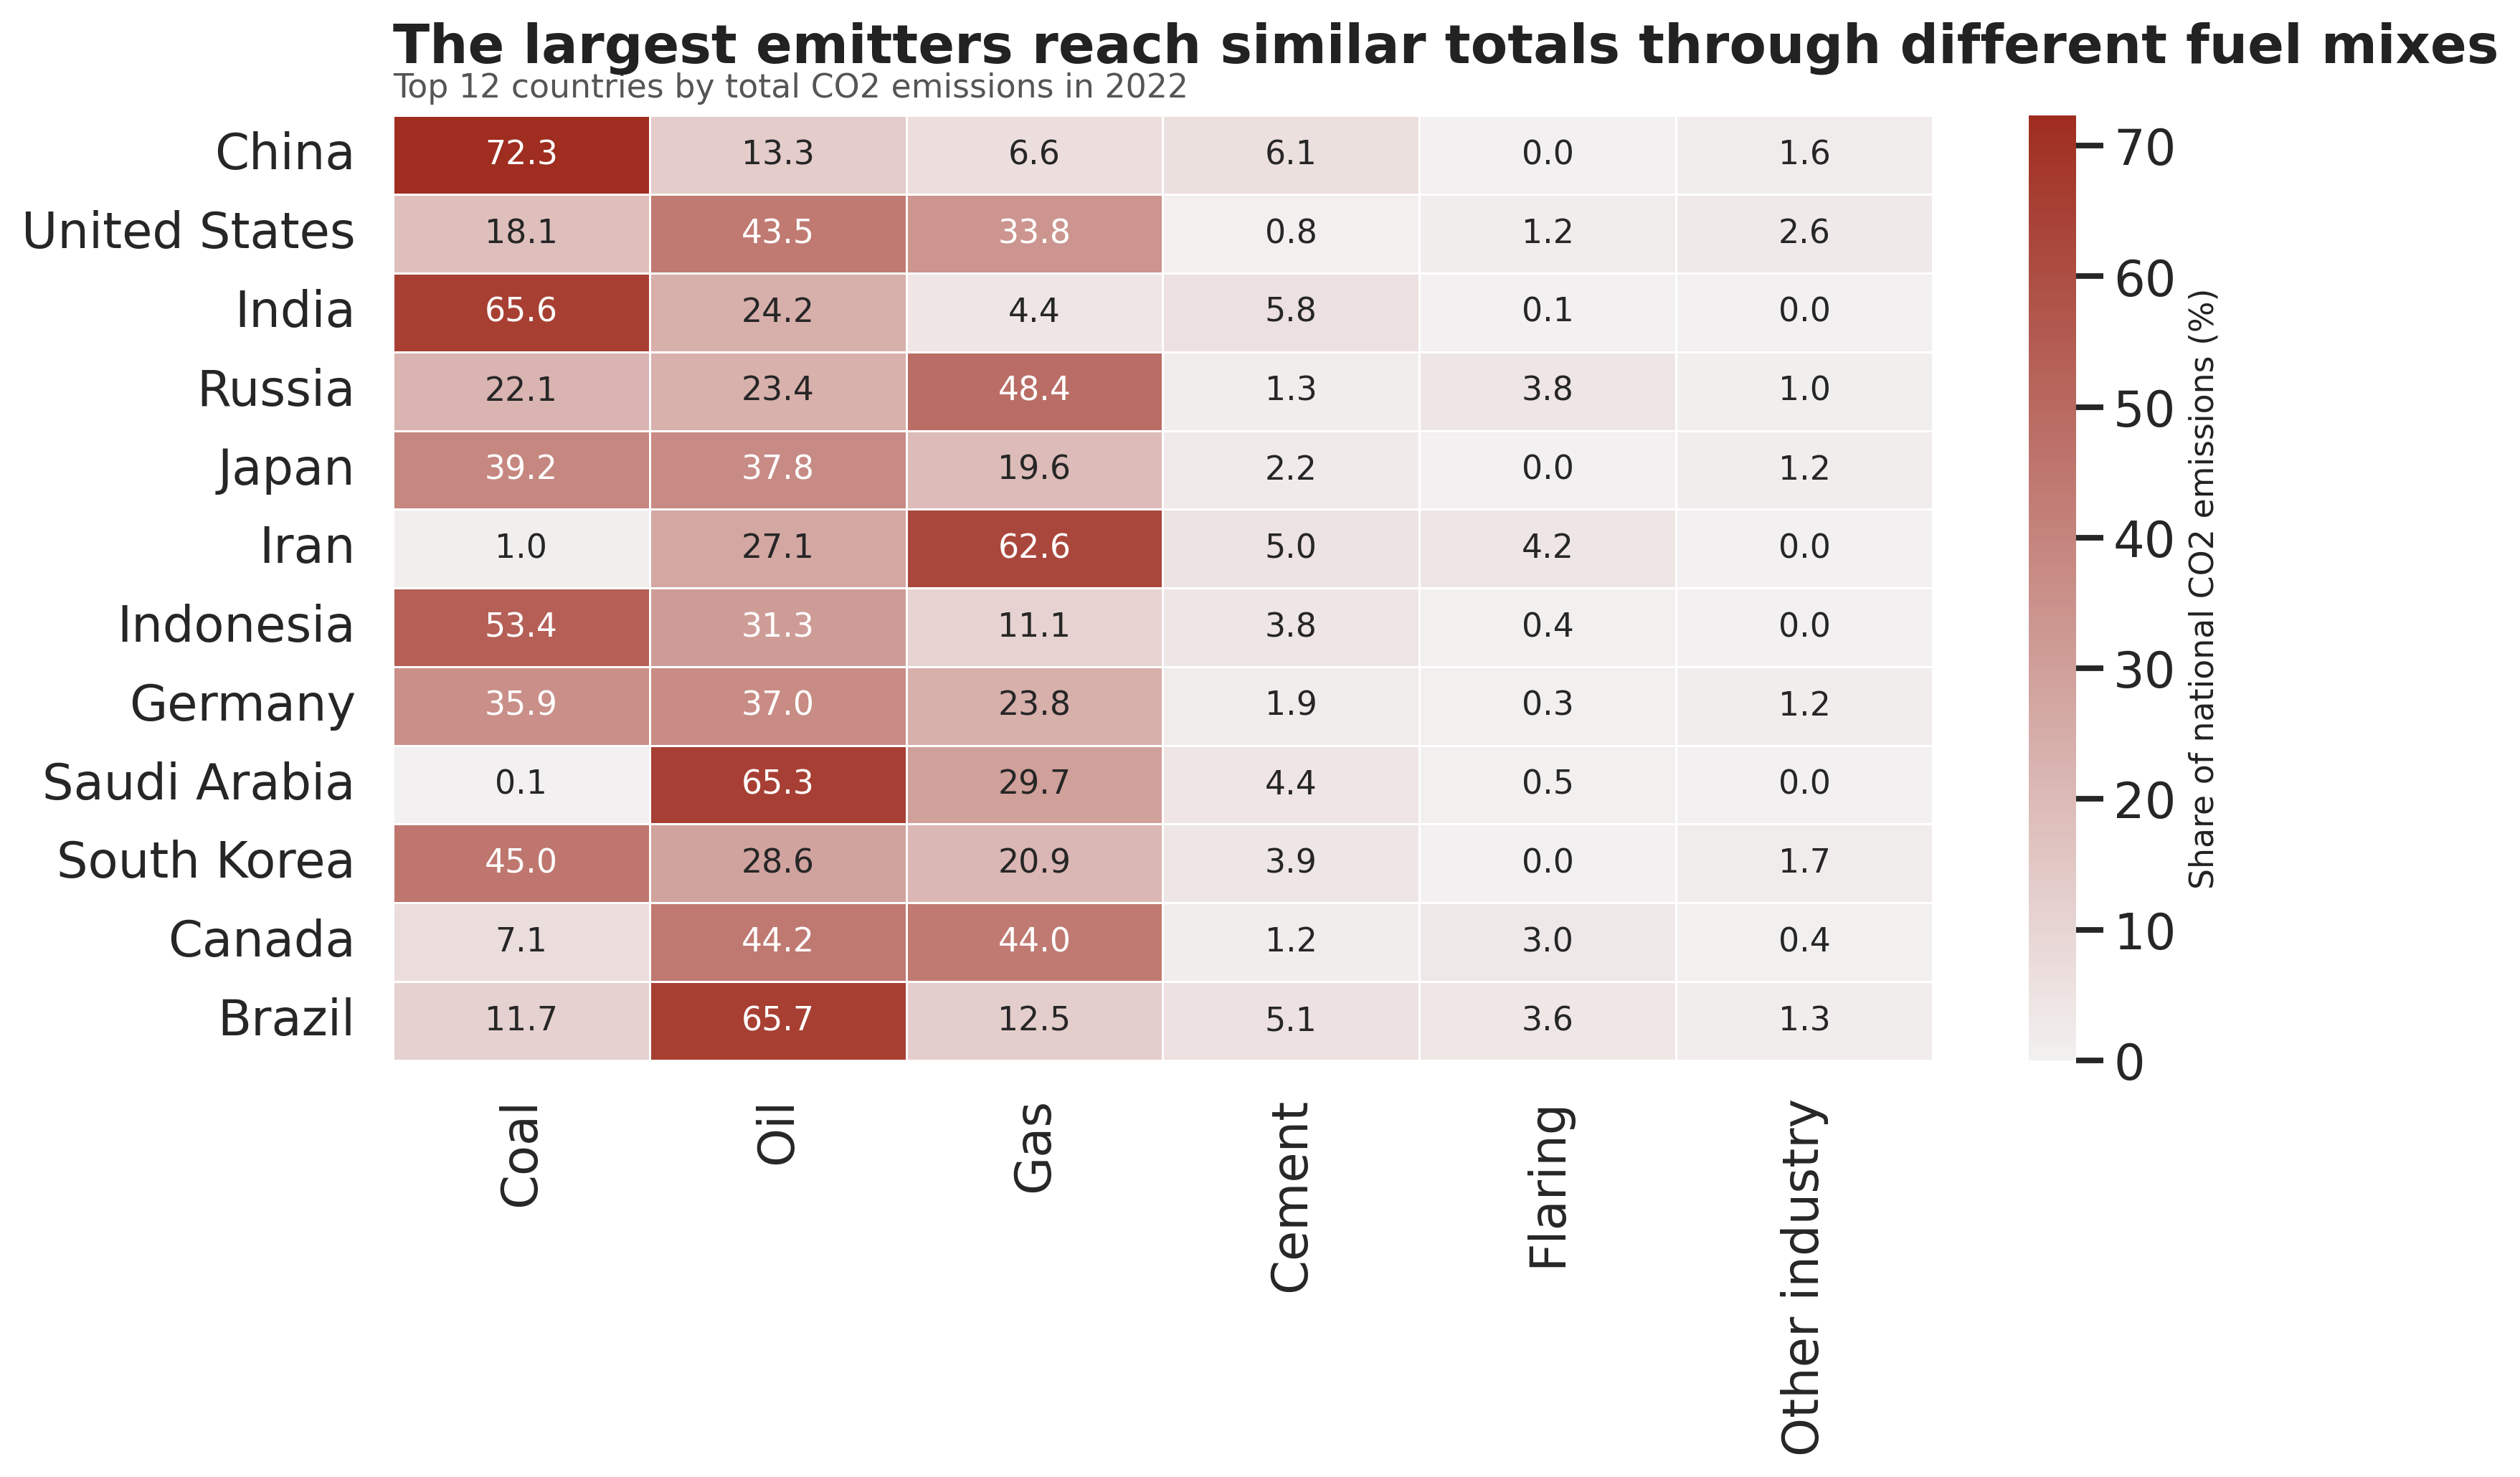
\includegraphics[width=\textwidth]{PS6c_Cheng.png}
\caption{Fuel-source composition of CO2 emissions among the 12 largest emitters in 2022.}
\end{figure}

Figure 3 focuses on the composition of emissions among the largest emitters.
China and India are much more coal-heavy than the United States, while Russia and Iran rely more on gas.
Saudi Arabia and Brazil are much more oil-heavy, which reflects their different energy structures.
This figure is helpful because two countries can have similarly large emissions totals while arriving there through very different fuels.
That matters for interpretation because policy tradeoffs depend on whether emissions come mainly from coal, oil, or gas.

\section*{Reproducibility}
The submitted Python file \texttt{PS6\_Cheng.py} reproduces the entire assignment.
On OSCER, the most direct way to reproduce the project is to run
\begin{quote}
\texttt{bash PS6\_Cheng.sh}
\end{quote}
which loads \texttt{Anaconda3/2023.03-1} on OSCER and then executes the Python script.
Equivalently, one can run
\begin{quote}
\texttt{module load Anaconda3/2023.03-1 \&\& python PS6\_Cheng.py}
\end{quote}
from the \texttt{PS6} directory.
These commands download the raw data, perform the cleaning steps described above, and export the three required PNG files:
\texttt{PS6a\_Cheng.png}, \texttt{PS6b\_Cheng.png}, and \texttt{PS6c\_Cheng.png}.

\end{document}
